\section{Implementation of the model}
\label{impl}

\subsection{Requirements}

%We want an agent able to coordinate its turn in real-time with the user in a real dialogue scenario. In this kind of interaction, 
Turn-taking management is one of the numerous processes an ECA has to manage to be engaged in a natural interaction with the user. 
Among others, turn-taking management is closely linked with 
the dialogue management, including natural language understanding and generation, 
the grounding which necessicates to generate and to react to the different types of feedback the user can produce, such as backchannels, 
and also the control of the engagement witht the user. 
Existing ECA architectures provide the core functionalities required to support these process, at least partially. 
Our aim was to propose a solution for integrating our model into existing ECA architecture.
However, the continuous nature of the two main components of the model that are executed in parallel, implies some adaptation of existing architectures. 

%and to bring a stone to the buiding of ECA able to sustain mixed initiative dialogue in a very human-like fashion. 

%For example, apart from the turn-taking coordination, the agent has to be able to interpret the utterance of the user, formulated in natural language, and to generate an utterance in response, managing grounding by interpreting and generating the different types of feedback the user can produce, such as backchannels, perceiving the engagement of the user or showing its own engagement in the dialogue. 
%In order to manage the concurrent execution of all these processes, we would like to use an existing modular architecture, where we could integrate our turn-taking model without adapting it to work with the other components of this architecture.

%On the contrary, our model perceives and controls the actions of the agent in a continuous fashion : actions of the agent are continuously modulated rather than triggered by decision modules, and the perception and decision processes run concurrently rather than sequentially. 
%These requirements follows the design principle of the recent architecture ASAP. 
%We thus chose the ASAP framework as a basis for the implementation of our model. 

The closest solution suitable for implementing our model is ASAP from \cite{kopp_architecture_2014}.
Nevertheless, some mandatory details lack in the specification of the ASAP architecture. For instance, we need to specify how to manage the concurrent execution of the different decision modules. Several conflicting actions can, for example be sent at the same time to the realizer, which thus necessitates a mechanism to select or merge the actions in order to avoid inconsistencies in the action generation. Another issue is the selection of the multimodal communicative actions from the commands provided by the decision modules, and specifically, how to deal with cases where these commands require to change in real-time the actions generated by the agent. 
%To address these issues we based our solution 
%We wanted also to specify more precisely the communication mecanism between the different modules.
We inspired from some principles of the Ymir architecture to address these issues and extended the ASAP architecture.  
%We will now describe our agent architecture.

\subsection{Architecture overview}

%We used the current repartition given by the ASAP architecture. 
The overall organisation of the architecture, which is composed of six modules, is shown on Figure \ref{overall_archi}. 
Modules dedicated to the perception are: 
the Sensing module receiving sensory data, 
the Behavior Interpreter module, interpreting behavioral patterns such as nodding from the multimodal sensory data, 
and the Function Interpreter, interpreting the communicative functions of the behavioral patterns. 
The decision part is composed of three modules, 
the Intent Planner generating the communicative intentions of the agent, 
the Behavior Planner generating the multimodal actions from the communicative intentions and managing the execution of the actions (activating, modulating or interrupting the actions) based on the behavioral patterns perceived by the Behavior Interpreter,
and finally the Behavior realizer. 
% COMMENT TODO: Pierre : Mathieu verifie les fonctions du behavior planner et du behavior realizer
% TODO: valider nom Behavior Interpreter (au lieu de Interpretation)

\begin{figure}
  \centering
  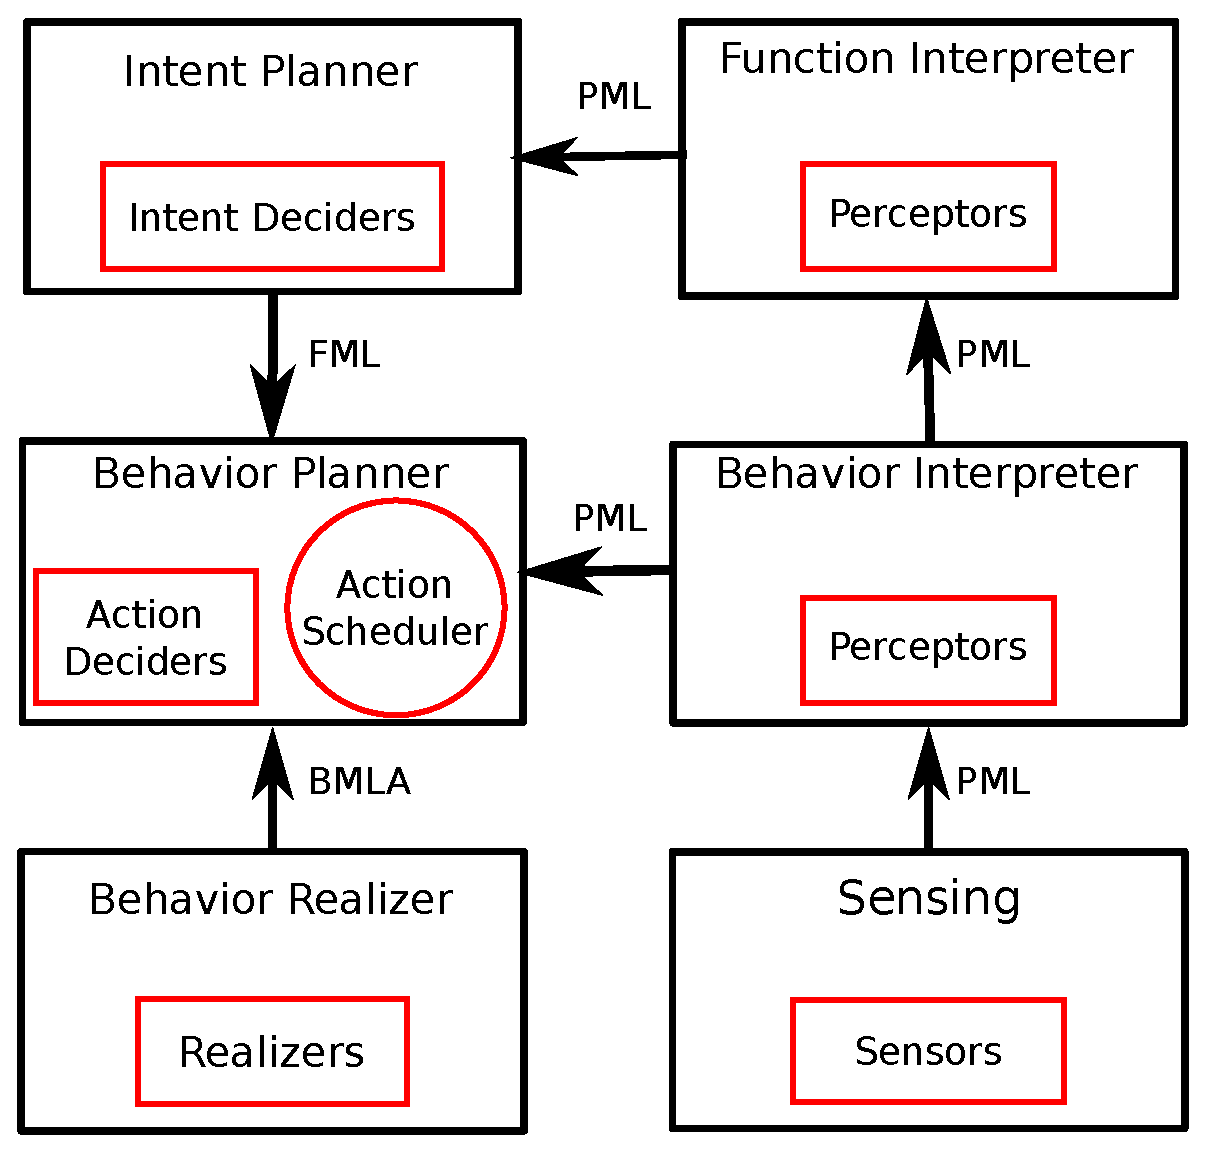
\includegraphics[width=\linewidth]{figure/impl_schema.eps}
  \caption{Overall organization of the architecture.}
  \label{overall_archi}
\end{figure}

Inside each modules, we divided the action control and perception into several submodules, each specialized into the perception of one particular behavioral pattern or communicative act, or into the generation or the control of one particular communicative intention. Following the terminology of \cite{thorisson_mind_1999}, the submodules of the behavior and function interpretation modules were called perceptors, those of the sensing modules the sensors, those of the intent planner and the behavior planner the deciders, and those of the behavior realizer were called realizers. 
Following the Ymir principles, the different submodules run concurrently, each submodule having its own execution frequency. The different execution frequencies will be defined when we will present the implementation of the model. The submodules are also either activated or deactivated like is Ymir.
%following \citep{thorisson_mind_1999}, defining if the submodules currently run (activated) in the architecture or not (deactivated). 
The activation or deactivation of modules depend on the current state of the dialog. 
For instance, modules involved in the detection of backchannels are activated only when the agent is the current speaker. 
The activation or deactivation of the submodules is implemented in the Function interpreter module by so-called module managers. 

We distinguish two types of decider: intention and action deciders. 
Intention deciders belong to the intent planner, and are responsible for the generation of the communicative intentions, based on the perception data provided by the function interpretation module. Intention deciders output FML data. 
The action deciders take as input the communicative intentions provided by the intention deciders, and the perceptual data provided by the behavior interpretation module. As output, they generate an action command that describes the action to control and the new values of the action parameters, according to the perceptual data and the agent's communicative intention. 
These commands are then sent to an action scheduler that have the responsibility to transcribe the commands into multimodal motor commands and to manage their concurrent execution. Once the motor commands have been determined, the action scheduler sends them to the realizers. 
We inspired from the Ymir architecture for the conception of the action scheduler. The difference is linked to the management of the continuous multimodal actions: the deciders modulating the actions of the agent, send to the action scheduler a continuous flow of commands. Our action scheduler manages this continuous flow of commands, with the capability of modifying on the fly the multimodal motor commands bound to a particular action, based on the parameters the deciders send to the action scheduler. 
The action scheduler sends then the different motor commands to the corresponding realizers using the BML language. 

\subsection{Implementation}

%We now describe our we implemented the different components of our model in the architecture. We illustrate on the 

Figure \ref{impl_modules} illustrates how the different submodules are implemented in the architecture. 

\begin{figure}
  \centering
  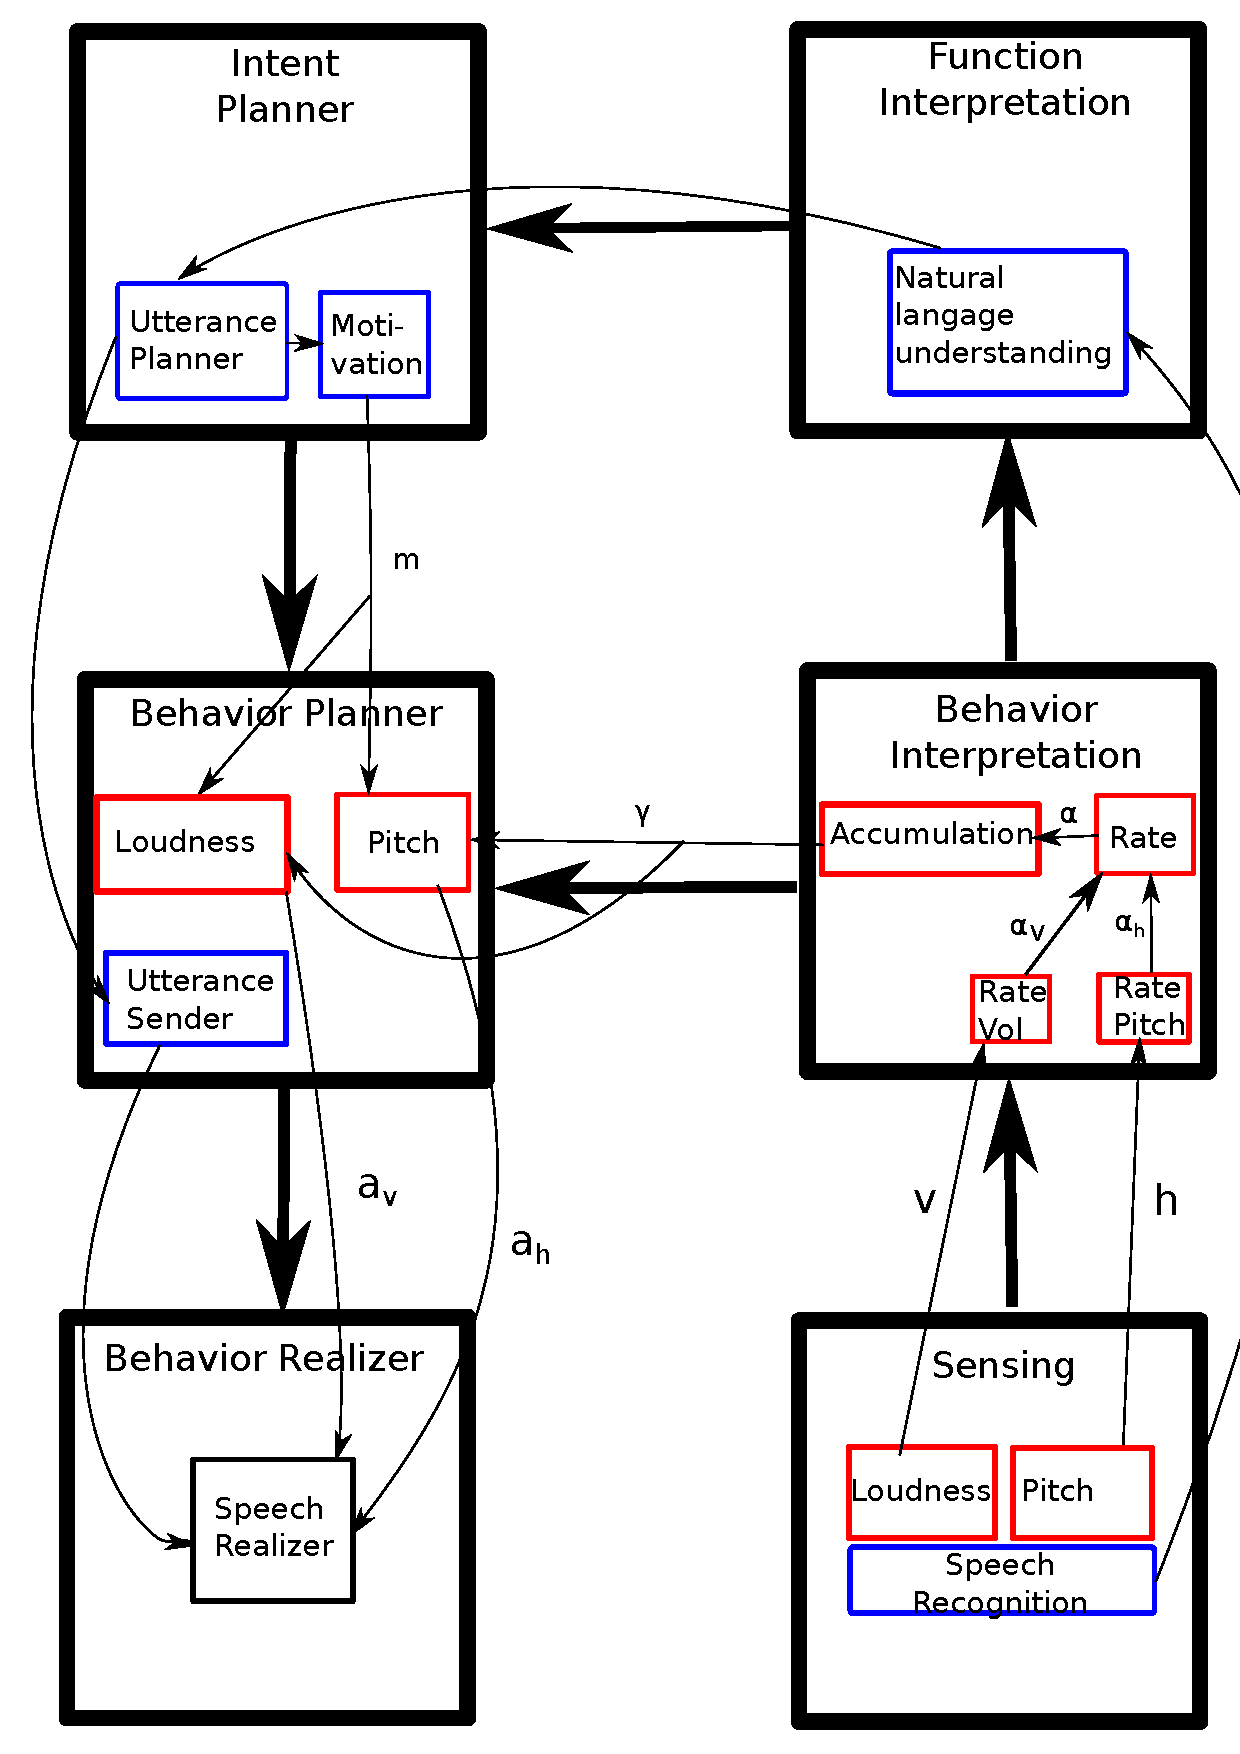
\includegraphics[width=\linewidth]{figure/impl_equ_dial.pdf}
  \caption{Distribution of the components of the model and the different submodules dedicated to the utterance interpretation and generation and the determination of the motivation value.}
  \label{impl_modules}
\end{figure}

%\subsubsection{Components of the model}
\subsubsection{Perceptual decision-making process}

%The two components of our model are implemented into two different modules of the architecture. 
According to our model, the agent is continuously collecting information about the user behavior. This information is a set of characteristics computed in real-time from the data the agent is able to sense, which is used to accumulation rate $\alpha(t)$. 
Each partial accumulation function $\alpha_j(t)$ is computed in a separate submodule (perceptor). The values computed by these modules are then summed in a dedicated perceptor according to Equation \ref{perc_int} which makes it available for the Behavior Planner. 

%Each signal the agent can perceived is  % produces a certain behavioral pattern that the agent has to discriminate. In this sense, 
%the user behavior perception component of our model should be implemented in the behavior interpretation module. We separate the user behavior perception component into several independant submodules. First, several submodules compute the partial accumulation rate for each signal produced by the user. These partial accumulation rates are then used by a submodule computing the global accumulation rate ($\alpha(t)$ variable in the model). This global accumulation rate is then used by the submodule in charge of updating the accumulation value according to the equation \ref{perc_int}. 
%The accumulation value is then sent to the behavior planner. 

\subsubsection{Production of the verbal ans non verbal signals}

The corresponding components are implemented in the Behavior Planner. Each equation controlling the modulation of the verbal and nonverbal signals is implemented in a specific action decider (for instance, one for the pitch, one for the loudness and one for the direction of gaze). 
%Each signal control equation is implemented in a particular action decider, for an agent managing the pitch and loudness variations of the agent, we would have then two different deciders, one for the pitch and one for the loudness. 
%The fact that the agent can 
The independent control of the different signals may seem inconsistent. For example, when the loudness is null, the agent does not produce any sound and talking about pitch variation is a nonsense. However, remember that the equations of our model define more the control parameters of the different realizers and do not correspond to the real signal values. The consistency of these values comes from the 'physical' production of the signals by the realizers.
%The management of the different physical couplings that can exist is done by the different realizers . 
Each action decider has two inputs: the motivation $m(t)$ to change its role or not and the accumulation value $\alpha(t)$. 

% --------
\subsubsection{Management of the motivation}

The motivation to speak, or to listen, may come from different factors. If the agent is finishing its utterance and has nothing more to say, it is likely that its motivation to change role will be positive. On the opposite, its motivation will likely be negative. The strength of this motivation is regulated by different processes, for instance the interpersonal attitudes of the participants \citep{ter_maat_how_2010,ravenet_conversational_2015} or the importance and nature of the contribution made by the participant \citep{cafaro_effects_2016}. As the nature of the factors influencing the motivation to speak can be different, we chose to implement its computation in an independent module of the Intent planner. This module updates over time the motivation of the agent and then send an FML data specifying the new motivation value to the Behavior planner. 
The action deciders generate as outputs action commands specifying the control parameters of the agent's signals. Then, these commands are sent to the action scheduler that updates the motor commands of the agent and then sends the modifications to the corresponding realizers.

\subsubsection{Verbal production}

In addition to the submodules implementing our turn-taking model, we added submodules dedicated to the interpretation of the user's natural language in the function interpretation module and to the generation of utterances in the Intent planner. 
Once the utterance has been generated by the dedicated submodule, it is sent to a specific submodule of the Behavior planner. This submodule decides to send to the Action scheduler an action command specifying the utterance to say, depending on the constraint that applies to this utterance. When the communicative intention specifies that the utterance should be produced immediately, the utterance is sent directly to the action scheduler whether or not the text to speech system (TTS) is currently producing an utterance. As a result, when the realizer receives the utterance, it cancels the previous utterance and send the new utterance to the TTS system. On the contrary, when the communicative intention specifies that the utterance should be generated after the current one, the decider waits until the realizer send a feedback specifying that it has completed the production of the utterance.
When the realizer receives then command specifying the generation of an utterance, it verifies the loudness and pitch values sent by the action scheduler. When the loudness value is greater than a threshold, it transmits the utterance to the TTS system. Each time the realizer receives new commands specifying the loudness and pitch values, it sends the new values to the TTS system that modulates the prosody of the utterance being currently generated. When loudness value received by the realizer becomes lesser than a threshold, the realizer decides to pause the ongoing utterance production.

\subsubsection{Technical choices}

For this implementation, we focused first on the perception and modulation of the voice loudness and pitch. We defined the different equations based on observations we made on a corpus of human interactions. For more details about these equations, see \cite{jegou_continuous_2015}. For the implementation of the signal control submodules we used the Runge-Kutta 4 method and for computation of the accumulation value, the Euler-Maruyama method. 

The implementation of the architecture and the submodules has been realised in JAVA. We set the execution frequency for the different submodules to 10~Hz. 
We used openSmile \citep{eyben_recent_2013} for the captation of the user's loudness and pitch (acquisition frequency: 10 Hz). % It  mesures and sends every 100~ms the loudness and pitch value of the user. 
The agent's graphical representation and its animation has been implemented using Unity3D. 
%The character has for the moment two different animation, speaking and listening. Those animations are synchronized with the output of the TTS system, such as, when the TTS pronounce an utterance, the speak animation is played and when no utterance is pronounced the listening animation is played. 

%In order to be able to
For testing our model we needed to use incremental speech recognition and synthesis tools. Thanks to the incremental speech recognizer, the agent was able to formulate hypotheses on what the user is saying before the s/he has finished to speak. Based on the hypotheses, the agent can then plan early its own utterance and then, depending on its motivation, can choose to interrupt or not the user. For the incremental speech recognition we used the Microsoft Speech API. 
The incremental speech synthesis tools allowed to modify on the fly the properties of the utterance being pronounced by the agent, such as revising what the agent  is currently saying or modulating the prosody. We mostly used an incremental speech synthesis tools to be able to modulate the prosody of the utterance pronounced by the agent. For this, we used inpro\_iSS created by \cite{baumann_inpro_2012}. 

\subsubsection{Example of interactions}

We will now demonstrate two examples of real-time interactions between a user and the agent. In the first one, the user tried to barge in the agent while the latter was uttering a long sentence (Figures \ref{sc_1} and \ref{sc_2}). In the second one  (Figures \ref{sc_3} and \ref{sc_4}), the agent was answering to a user's question it had understood before the end of the user's turn. 
 
%In these examples, the agent was able to interpret the sentence pronounced by the user and to chose which sentence to utter in response to the user's utterance. 
For these experimental scenarios, we formulated adjacent pairs to determine which sentence the agent will say in response to the user's utterances. 
For each examples, we will show the loudness profile for the interaction transcription, represented as green curves and will show below the transcription of the dialog between the two participants. In the figures, the ``detect" annotation indicates when the agent was certain about the user's utterance and planed the utterance to be said. 


% --------- Fin lecture Pierre

Figure \ref{sc_1} corresponds to the first interaction when the agent had a strong motivation to keep the turn ($m_{loc}=-1.0$). 
As a result, the agent raised its loudness between the expression ``mount" and ``a shelf" and the loudness remained high until the agent pronounced the word ``red". This can be explained by an accumulation variable becoming positive when the user barged-in, meaning that the agent was perceiving that the user was trying to take the turn. This positive accumulation value is sent from the behavior interpreter module to the behavior planner. 
%The submodules controlling the agents actions raises then their attractors, making the control parameter raising and then finally making the loudness of the utterance of the agent raise. 
Contrarily, Figure \ref{sc_2} shows what happened when the agent had a weak motivation to keep on speaking, making it to release the turn before the end of its utterance in response to the user's signals variations.

\begin{figure}
  \centering
  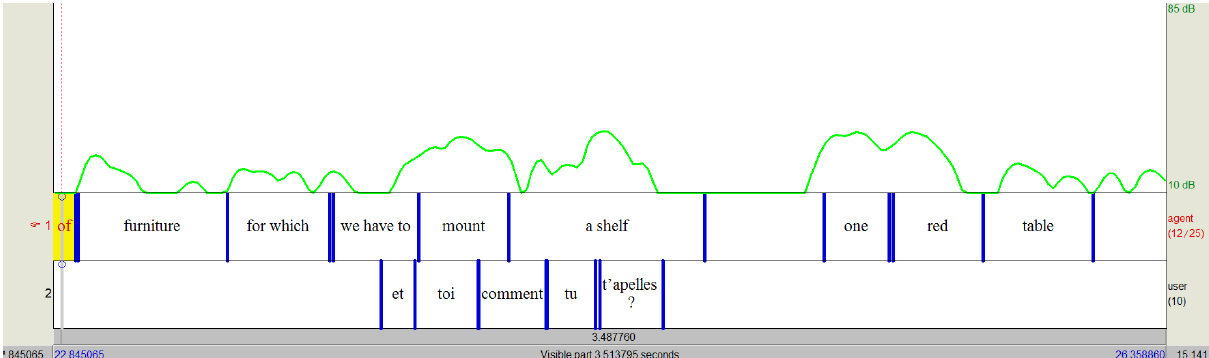
\includegraphics[width=\linewidth]{figure/volume_transcript_1_1.png}
  \caption{Illustration of the first interaction. The user tries here to barge-in the agent, the latter does not let the turn to the user.}
  \label{sc_1}
\end{figure}

\begin{figure}
\centering
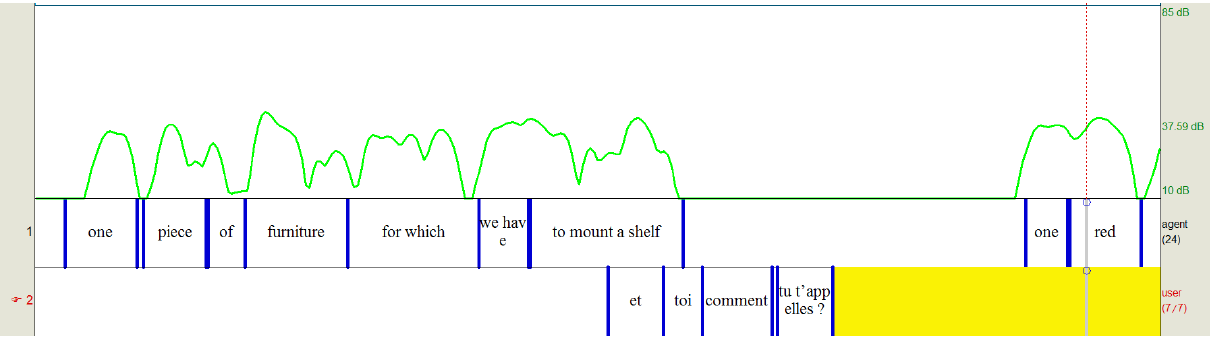
\includegraphics[width=\linewidth]{figure/volume_transcript_1_2.png}
\caption{Illustration of a scenario where the agent interrupts itself in response to the user barge-in.}
\label{sc_2}
\end{figure}

\begin{figure}
\centering
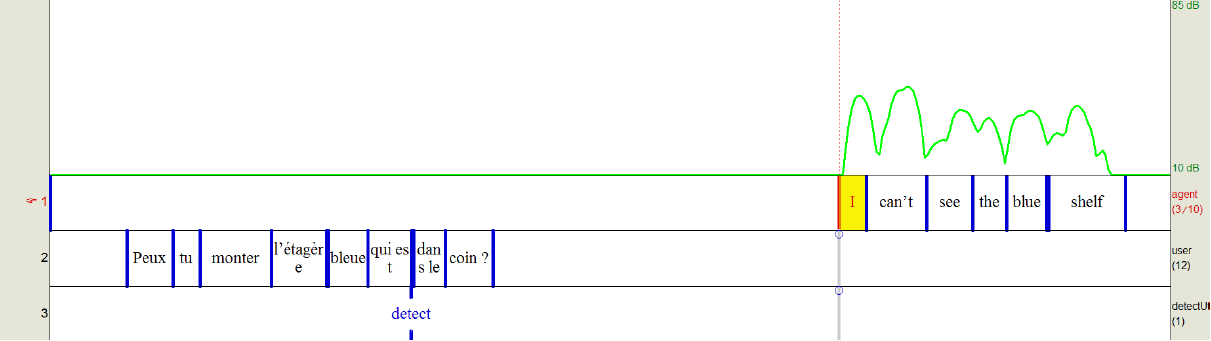
\includegraphics[width=\linewidth]{figure/volume_transcript_2_2.png}
\caption{Illustration of a scenario where the agent waits the end of turn of the user even if it has understood was the latter was saying.}
\label{sc_3}
\end{figure}

\begin{figure}
\centering
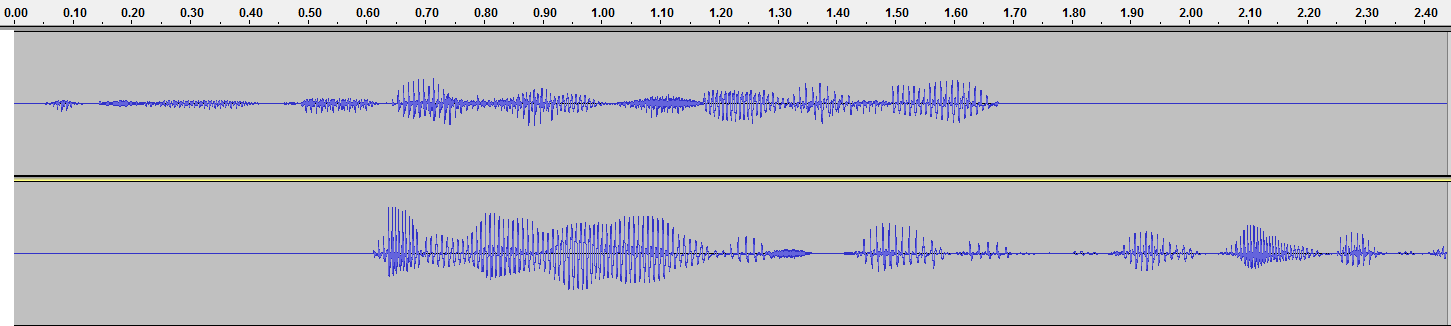
\includegraphics[width=\linewidth]{figure/volume_transcript_2_1.png}
\caption{Illustration of a scenario where the agent interrupts the user as soon as it has understood was the user was saying.}
\label{sc_4}
\end{figure}

Figure \ref{sc_3} illustrates the second interaction: the agent was the current listener and had a weak motivation to answer to the user's question, although it had understood what the user was saying before the end of the user's turn. In this situation, the agent did not start speaking before the end of the user's question. Figure \ref{sc_4} shows what happened in the same situation when the agent had a strong motivation to answer to the user's question. 

%shows an other example when the user asks a question to the agent, and then agent recognizes the utterance pronounced by the user before the latter has finished to pronounce it. Once the agent has recognized what the user was saying the agent wait the user finished its utterance before interrupting it. 

As soon as the agent had recognized what the user was saying, its utterance generation module planned an utterance that was sent to the realizer. Nevertheless, as the loudness command of the realizer was less than a given threshold, the utterance was not immediately launched in the TTS. 
The control parameter provided by the signal control submodules, the loudness parameter depends on the result of the turn-taking submodules. While the user is still speaking, the agent having here a weak motivation to speak, the loudness of the agent remains lesser than the threshold value. When the user has finished the turn, the accumulation value begins to raise towards positive value. When this accumulation value attain a certain (high) value, the agent raise the loudness attractor, making the loudness parameter sent to the realizer higher and higher. As soon as this loudness parameter received by the realizer becomes high than the silence threshold value, the utterance is launched in the realizer.
The fact the agent waits a certain amount of time in this scenario is due to the way we defined the loudness control equations. In these equations, depending on the motivation value, the loudness begin to rise after a certain accumulation value, the lowest the motivation, the higher the accumulation value needed to begin to raise the loudness. If we raise the motivation value, the agent will begin to speak sooner in the previous scenario, and, as an extreme, will interrupt the agent if the agent has a strong motivation value to speak that makes him not waiting a positive accumulation value before taking the turn as shown on the figure \ref{sc_4}. 
